% =====================================================================
%  PROPOSAL SKRIPSI FILKOM UB — BERKAS INDUK
%  Diadaptasi dari template tesis generik agar sesuai Panduan Skripsi
%  Filkom UB v3.0 (Calibri, spasi tunggal, "Landasan Kepustakaan").
%
%  Kompilasi (WAJIB XeLaTeX — bukan pdflatex — karena pakai fontspec):
%    xelatex -interaction=nonstopmode main_proposal.tex   (jalankan 2x)
%
%  Struktur:
%    preamble.tex                ← paket & style, dipakai bareng main_skripsi.tex
%    frontmatter/cover.tex       ← cover (label "PROPOSAL SKRIPSI" diisi di bawah)
%    chapters/bab1–bab3.tex      ← Pendahuluan, Landasan Kepustakaan, Metodologi
%    backmatter/referensi.tex    ← daftar pustaka (Harvard, gaya UB)
%
%  Cakupan proposal skripsi Filkom UB = Bab 1–3 + Daftar Referensi.
%  Lampiran dihapus dari cakupan (Iterasi 10 item 4) -- backmatter/lampiran.tex
%  masih ada di repo tapi tidak lagi di-\include (lihat CATATAN_PERBAIKAN.md).
%  Bab 4 dst. baru ditulis setelah proposal disetujui pembimbing — build
%  itu ada di main_skripsi.tex, bukan berkas ini.
% =====================================================================

% !TEX root = main_proposal.tex
% =====================================================================
%  PREAMBLE BERSAMA — dipakai oleh main_proposal.tex dan main_skripsi.tex
%  (\input dari kedua entry point supaya paket/style tidak dobel-tulis)
% =====================================================================

\documentclass[12pt,a4paper]{report}

% ── Bahasa & font ────────────────────────────────────────────────────
\usepackage[indonesian]{babel}   % otomatis: Bab / Gambar / Tabel / Daftar Isi
\usepackage{fontspec}            % wajib XeLaTeX/LuaLaTeX, bukan pdflatex
% Calibri terpasang di sistem ini, jadi dipakai langsung -- ini font yang
% diwajibkan Panduan Skripsi Filkom UB v3.0 (Lampiran A.3), bukan sekadar
% pengganti. Kalau compile di mesin lain yang TIDAK punya Calibri (mis.
% Overleaf, Linux, atau Mac tanpa MS Office), ganti "Calibri" -> "Carlito"
% pada baris \setmainfont di bawah -- itu pengganti metrik-kompatibel
% resmi untuk Calibri (dipakai LibreOffice sebagai substitusinya),
% sehingga tata letak/line-break tetap identik.
\setmainfont{Calibri}
% Catatan: paket sansmathfonts (font matematika sans-serif) tidak tersedia
% di lingkungan kompilasi ini dan dihapus. Simbol matematika pada equation
% akan memakai font matematika default (Latin Modern Math, serif tipis)
% sementara badan teks tetap Calibri — ini perilaku standar LaTeX dan tetap
% rapi dibaca. Jika ingin font matematika sans-serif penuh, pasang paket
% "sansmath" atau "unicode-math" secara manual di sistem Anda.
\usepackage{setspace}
\singlespacing                   % spasi 1 — Panduan Skripsi Filkom UB v3.0, Lampiran A.4

% ── Jarak baris daftar tabel dan daftar gambar ───────────────────────────────────────────────
\usepackage{etoolbox}
\makeatletter
\patchcmd{\@chapter}{\addtocontents{lot}{\protect\addvspace{10\p@}}}{}{}{}
\patchcmd{\@chapter}{\addtocontents{lof}{\protect\addvspace{10\p@}}}{}{}{}
\makeatother

% ── Tata letak halaman ───────────────────────────────────────────────
\usepackage[a4paper,left=4cm,right=3cm,top=3cm,bottom=3cm]{geometry}
\setlength{\parindent}{1.27cm}
\setlength{\parskip}{8pt plus 2pt minus 2pt}   % jarak vertikal antarparagraf, mengikuti template resmi

% ── Kerapatan daftar bernomor/berpoin ────────────────────────────────
% enumitem dipakai supaya jarak antarbutir enumerate/itemize tidak ikut
% melebar akibat \parskip di atas -- tanpa ini, tiap butir daftar akan
% mendapat jarak sebesar \parskip juga, jauh lebih lebar dari yang wajar.
\usepackage{enumitem}
\setlist{itemsep=2pt, parsep=0pt, topsep=4pt, partopsep=0pt}

% ── Tabel & gambar ───────────────────────────────────────────────────
\usepackage{graphicx}
\graphicspath{{assets/}}
\usepackage{booktabs}
\usepackage{array}
\usepackage{multirow}
\usepackage{longtable}
\usepackage{float}
\usepackage{caption}
% Semua caption: bold label, centered, posisi default (bawah untuk gambar, atas untuk tabel)
\captionsetup{font=normalsize, labelfont=bf, textfont=bf, justification=centering, singlelinecheck=false, labelsep=space}
\captionsetup[figure]{position=below}
\captionsetup[table]{position=above}

% ── Tipe float kustom (ganti nama caption sesuai kebutuhan) ──────────
% Contoh: \DeclareCaptionType{diagram}[Diagram][Daftar Diagram]
% Contoh: \DeclareCaptionType{bagan}[Bagan][Daftar Bagan]
% Setelah deklarasi, gunakan environment {diagram} seperti {figure}
%   \begin{diagram}[H]
%     \centering
%     \includegraphics[width=\textwidth]{nama_file}
%     \caption{Judul diagram}
%   \end{diagram}

% ── Tabel full-border, boleh sambung ke halaman berikutnya ───────────
% Iterasi 10 item 11: semua tabel pakai longtable (bukan table+tabular)
% supaya baris otomatis lanjut ke halaman berikutnya kalau kepanjangan,
% dengan header berulang di tiap halaman lanjutan. Garis vertikal
% (|c|c|) dan \hline di tiap baris dipertahankan di semua tabel --
% booktabs/adjustbox TIDAK dipakai lagi untuk tabel isi bab.
% Template:
%   \begin{longtable}{|p{4cm}|p{9cm}|}
%     \caption{Judul Tabel}
%     \label{tab:label} \\
%     \hline
%     \textbf{Kolom 1} & \textbf{Kolom 2} \\ \hline
%     \endfirsthead
%     \hline
%     \textbf{Kolom 1} & \textbf{Kolom 2} \\ \hline
%     \endhead
%     \hline
%     \endfoot
%     \hline
%     \endlastfoot
%     Isi baris & Isi baris \\ \hline
%   \end{longtable}

% ── Matematika ───────────────────────────────────────────────────────
\usepackage{amsmath}
\numberwithin{equation}{chapter}   % nomor persamaan per-bab: (3.1), (3.2)
\usepackage{amssymb}
\usepackage{siunitx}
\sisetup{output-decimal-marker={,}}

% ── Heading bab & subbab ─────────────────────────────────────────────
\usepackage{titlesec}
\usepackage{indentfirst}         % inden paragraf pertama juga (bukan cuma paragraf ke-2 dst),
                                  % standar konvensi Indonesia -- default LaTeX tidak begini
% Bab: "BAB X JUDUL" satu baris, centered, bold, normal size
% CATATAN: JANGAN pakai shape [block] di sini -- kombinasi [block] + \chapter
% di kelas report bikin \tableofcontents/\listoffigures/\listoftables render
% KOSONG (isi .toc/.lof/.lot tetap benar, cuma tidak ke-render ke halaman).
% Tanpa opsi shape (default titlesec), tampilan visualnya identik tapi TOC
% normal. Sudah diverifikasi lewat isolasi bug, jangan tambahkan [block] lagi.
% Ukuran font heading (Iterasi 10 item 4): bab 16pt, subbab 14pt, sub-subbab 12pt
\titleformat{\chapter}
  {\normalfont\fontsize{16}{20}\selectfont\bfseries\centering}
  {BAB \thechapter\space}
  {0pt}
  {\MakeUppercase}
\titlespacing*{\chapter}{0pt}{-40pt}{20pt}
% Subbab: "X.Y Judul" bold, left-aligned, jarak label-judul normal
\titleformat{\section}
  {\normalfont\fontsize{14}{17}\selectfont\bfseries}
  {\thesection}
  {1em}
  {}
\titleformat{\subsection}
  {\normalfont\fontsize{12}{15}\selectfont\bfseries}
  {\thesubsection}
  {1em}
  {}

% \titleformat{\chapter} above only reliably restyles the NUMBERED form.
% \chapter* (used by \tableofcontents/\listoffigures/\listoftables and by
% "Daftar Referensi") falls back to the class's own \@makeschapterhead,
% which is left-aligned/not-uppercase by default -- Iterasi 10 item 1
% flagged exactly this mismatch against "BAB 1 PENDAHULUAN"'s style.
% Redefine it directly so every unnumbered chapter heading matches: centered,
% same 16pt size, uppercase, same 20pt space-after as numbered chapters.
\makeatletter
\renewcommand{\@makeschapterhead}[1]{%
  {\parindent\z@ \centering \normalfont\fontsize{16}{20}\selectfont\bfseries
   \MakeUppercase{#1}\par\nobreak\vskip 20pt}%
}
\makeatother

% ── Daftar Isi / Daftar Gambar / Daftar Tabel ────────────────────────
\usepackage{tocloft}
% Tanpa bold di semua entri (termasuk level bab, yang default-nya bold)
\renewcommand{\cftchapfont}{\normalfont}
\renewcommand{\cftchappagefont}{\normalfont}
% Entri bab di daftar isi ikut menuliskan "BAB X", sama seperti heading aslinya
\renewcommand{\cftchappresnum}{BAB\space}
\setlength{\cftchapnumwidth}{3em}
% Titik-titik penghubung ke nomor halaman juga muncul di level bab
% (default kelas report: level bab tanpa titik-titik, cuma section ke bawah)
\renewcommand{\cftchapdotsep}{\cftdotsep}
% Titik-titik lebih rapat di semua level
\renewcommand{\cftdotsep}{1}
% Jarak vertikal antarentri dipersempit lagi (Iterasi 13 item 1 -- 2pt masih
% dirasa lebar setelah dicoba) -- 0pt di semua level: bab (Daftar Isi),
% gambar (Daftar Gambar), tabel (Daftar Tabel), dan section (baris "X.Y
% Judul" di dalam Daftar Isi, belum pernah disentuh sebelumnya)
\setlength{\cftbeforechapskip}{0pt}
\setlength{\cftbeforefigskip}{0pt}
\setlength{\cftbeforetabskip}{0pt}
\setlength{\cftbeforesecskip}{0pt}

% ── Mikrografi & hyperlink ───────────────────────────────────────────
\usepackage{microtype}
\setlength{\emergencystretch}{3em}
\usepackage{url}                 % \url{} bisa memecah baris di URL/DOI panjang
\PassOptionsToPackage{hyphens}{url}
\usepackage[hidelinks]{hyperref}
\hypersetup{
  pdftitle={Pengaruh Skema Pembagian Data Berbasis Film pada Dataset E-SERAVD terhadap Performa Klasifikasi Pengenalan Emosi Ucapan Berbahasa Indonesia},
  pdfauthor={Gaung Taqwa Indraswara},
}

% ── Warna ────────────────────────────────────────────────────────────
\usepackage{xcolor}
\definecolor{cProses}{HTML}{4A6D8C}    \definecolor{cProsesBg}{HTML}{DCE6F0}
\definecolor{cData}{HTML}{8C7B4A}      \definecolor{cDataBg}{HTML}{F0EBDC}
\definecolor{cKeputusan}{HTML}{8C6A4A} \definecolor{cKeputusanBg}{HTML}{F5E9D8}
\definecolor{cTerm}{HTML}{4A4A4A}      \definecolor{cTermBg}{HTML}{E4E4E4}
\definecolor{cGrup}{HTML}{9AA7B4}      \definecolor{cGrupBg}{HTML}{F2F5F8}
\definecolor{cOk}{HTML}{3E7D5A}        \definecolor{cOkBg}{HTML}{DFF0E6}
\definecolor{cBad}{HTML}{A4503C}       \definecolor{cBadBg}{HTML}{F2DED7}
\definecolor{kodeBg}{HTML}{F7F7F4}
\definecolor{kodeKomentar}{HTML}{5A7D5A}
\definecolor{kodeKunci}{HTML}{4A4A8C}
\definecolor{kodeString}{HTML}{8C5A3C}

% ── TikZ / pgfplots ──────────────────────────────────────────────────
\usepackage{tikz}
\usepackage{pgfplots}
\pgfplotsset{compat=1.18}
\usetikzlibrary{
  shapes.geometric, arrows.meta, positioning,
  calc, fit, backgrounds, decorations.pathreplacing
}

% node styles (flowchart monokrom)
\tikzset{
  term/.style={ellipse, draw=black, line width=.5pt,
    minimum width=26mm, minimum height=9mm,
    align=center, font=\footnotesize},
  proc/.style={rectangle, draw=black, line width=.5pt,
    minimum width=34mm, minimum height=11mm,
    inner xsep=3.4mm, align=center, font=\footnotesize,
    append after command={\pgfextra{
      \draw[line width=.5pt]
        ([xshift=1.6mm]\tikzlastnode.north west)
        -- ([xshift=1.6mm]\tikzlastnode.south west);
      \draw[line width=.5pt]
        ([xshift=-1.6mm]\tikzlastnode.north east)
        -- ([xshift=-1.6mm]\tikzlastnode.south east);}}},
  procplain/.style={rectangle, draw=black, line width=.5pt,
    minimum width=34mm, minimum height=11mm,
    align=center, font=\footnotesize},
  io/.style={trapezium, trapezium left angle=70, trapezium right angle=110,
    draw=black, line width=.5pt,
    minimum width=28mm, minimum height=9mm,
    align=center, inner sep=2pt, font=\footnotesize},
  dec/.style={diamond, aspect=2, draw=black, line width=.5pt,
    align=center, inner sep=1pt, font=\footnotesize},
  arr/.style={-{Stealth[length=2.2mm]}, draw=black, line width=.5pt},
  flbl/.style={font=\footnotesize, fill=white, inner sep=1pt},
}

% ── Listing kode ─────────────────────────────────────────────────────
\usepackage{listings}
\renewcommand{\lstlistingname}{Kode Sumber}
\lstdefinestyle{kode}{
  backgroundcolor=\color{kodeBg},
  basicstyle=\ttfamily\footnotesize,
  commentstyle=\color{kodeKomentar}\itshape,
  keywordstyle=\color{kodeKunci}\bfseries,
  stringstyle=\color{kodeString},
  numberstyle=\ttfamily\scriptsize\color{gray},
  numbers=left, numbersep=8pt, stepnumber=1,
  frame=single, rulecolor=\color{cGrup},
  breaklines=true, breakatwhitespace=false,
  showstringspaces=false, tabsize=2,
  captionpos=t, xleftmargin=18pt, framexleftmargin=14pt,
  literate={→}{$\rightarrow$}{1} {≤}{$\le$}{1} {≥}{$\ge$}{1}
           {×}{$\times$}{1} {—}{{-{}-}}1 {–}{{-}}1
}
\lstset{style=kode}

% ── Makro bantu ──────────────────────────────────────────────────────
\usepackage[export]{adjustbox}
\newcommand{\gambarbesar}[1]{%
  \adjustbox{max width=\textwidth, max totalheight=0.82\textheight, center}{#1}}

% ── Jenis dokumen (diisi beda oleh main_proposal.tex / main_skripsi.tex) ──
% \doctypelabel: label besar di cover ("PROPOSAL SKRIPSI" atau "SKRIPSI").
% \doctypesubtitle + \ifdoctypesubtitle: baris kecil di bawahnya, cuma
% dipakai skripsi penuh -- boolean-nya yang menentukan baris itu dicetak
% atau tidak (bukan sekadar dikosongkan), supaya versi proposal tidak
% menyisakan jarak kosong dari baris yang seharusnya tidak ada.
\newcommand{\doctypelabel}{}
\newcommand{\doctypesubtitle}{}
\newif\ifdoctypesubtitle
\doctypesubtitlefalse

% ── Metadata dokumen ─────────────────────────────────────────────────
\title{Pengaruh Skema Pembagian Data Berbasis Film pada Dataset E-SERAVD
  terhadap Performa Klasifikasi Pengenalan Emosi Ucapan Berbahasa Indonesia}
\author{Gaung Taqwa Indraswara}
\date{\the\year}

\renewcommand{\doctypelabel}{PROPOSAL SKRIPSI}

\begin{document}

% ── Cover (tidak bernomor halaman) ───────────────────────────────────
\pagenumbering{gobble}
% =====================================================================
%  HALAMAN JUDUL (COVER)
%  Ganti semua teks dalam kurung siku [ ] sesuai data Anda.
% =====================================================================

\begin{titlepage}
\centering

% ── Judul ─────────────────────────────────────────────────────────────
\vspace*{1cm}
{\normalsize\bfseries Analisis Pengaruh Strategi Fine-Tuning Dua Tahap
  terhadap Akurasi Pengenalan Emosi Ucapan Berbahasa Indonesia}\\[1.2cm]

% ── Jenis karya (diisi oleh main_proposal.tex atau main_skripsi.tex) ──
{\normalsize\bfseries \doctypelabel}\\[0.3cm]
{\normalsize \doctypesubtitle}\\[2.2cm]

% ── Penulis ───────────────────────────────────────────────────────────
{\normalsize Disusun oleh:}\\[0.2cm]
{\normalsize Gaung Taqwa Indraswara}\\[0.1cm]
{\normalsize NIM: 235150207111043}\\[2.5cm]

% ── Logo ──────────────────────────────────────────────────────────────

\includegraphics[width=5cm]{assets/ub-logo-small.png}\\[2.5cm]

% ── Institusi (all caps) ──────────────────────────────────────────────
{\normalsize PROGRAM STUDI TEKNIK INFORMATIKA}\\[0.15cm]
{\normalsize DEPARTEMEN TEKNIK INFORMATIKA}\\[0.15cm]
{\normalsize FAKULTAS ILMU KOMPUTER}\\[0.15cm]
{\normalsize UNIVERSITAS BRAWIJAYA}\\[0.15cm]
{\normalsize MALANG}\\[0.15cm]
{\normalsize 2026}

\end{titlepage}
\clearpage


% ── Front matter (nomor halaman romawi) ──────────────────────────────
% Menurut Panduan Skripsi Filkom UB v3.0, proposal skripsi hanya mencakup
% Pendahuluan, Landasan Kepustakaan, Metodologi, Daftar Referensi, dan
% Lampiran A/B — TANPA lembar pengesahan, pernyataan orisinalitas,
% abstrak, atau kata pengantar (elemen-elemen itu khas skripsi final
% pasca-sidang; lihat main_skripsi.tex untuk versi itu).
\pagenumbering{roman}
\setcounter{page}{1}

% Daftar Isi/Gambar/Tabel dipanggil manual (bukan \tableofcontents dkk. polos)
% karena paket tocloft menggantikan mekanisme heading ketiga perintah itu
% sendiri dan TIDAK ikut gaya \titleformat{\chapter} (16pt, center, uppercase)
% seperti "BAB 1 PENDAHULUAN"/"DAFTAR REFERENSI" -- Iterasi 10 item 1.
% \@starttoc{<ext>} adalah bagian dari \tableofcontents dkk. yang membaca isi
% berkas .toc/.lof/.lot; heading di atasnya sekarang ditulis manual sendiri.
% \clearpage eksplisit di antara ketiganya (Iterasi 12 item 1) -- tocloft
% tidak clearpage otomatis seperti \chapter*, jadi tanpa ini Daftar Gambar
% dan Daftar Tabel bisa berbagi satu halaman kalau Daftar Gambar pendek.
% Entri TOC-nya sendiri juga di-\MakeUppercase (Iterasi 12 item 2).
\makeatletter
{\centering\normalfont\fontsize{16}{20}\selectfont\bfseries
  \MakeUppercase{Daftar Isi}\par\nobreak\vskip 20pt}
\addcontentsline{toc}{chapter}{\MakeUppercase{Daftar Isi}}
\@starttoc{toc}

\clearpage
{\centering\normalfont\fontsize{16}{20}\selectfont\bfseries
  \MakeUppercase{Daftar Gambar}\par\nobreak\vskip 20pt}
\addcontentsline{toc}{chapter}{\MakeUppercase{Daftar Gambar}}
\@starttoc{lof}

\clearpage
{\centering\normalfont\fontsize{16}{20}\selectfont\bfseries
  \MakeUppercase{Daftar Tabel}\par\nobreak\vskip 20pt}
\addcontentsline{toc}{chapter}{\MakeUppercase{Daftar Tabel}}
\@starttoc{lot}
\makeatother

\clearpage
\pagenumbering{arabic}
\setcounter{page}{1}

% ── Bab-bab utama ────────────────────────────────────────────────────
% !TEX root = ../main_proposal.tex
% =====================================================================
%  BAB 1 — PENDAHULUAN
% =====================================================================

\chapter{\MakeUppercase{Pendahuluan}}

\section{Latar Belakang}
\label{sec:1.1}

Emosi merupakan komponen mendasar dalam komunikasi antarmanusia, karena
emosi memungkinkan seseorang menyampaikan maksud dan keadaan batin
secara lebih utuh daripada makna literal kata-kata. Dalam interaksi
manusia dan mesin, pengenalan emosi dari sinyal ucapan memegang peranan
penting bagi pengembangan komputasi afektif dan sistem interaktif yang
mampu merespons pengguna secara lebih personal (Dar and Delhibabu,
2024). Karakteristik inilah yang mendasari berkembangnya \emph{speech
emotion recognition} (SER), yaitu bidang kajian yang berupaya mengenali
kondisi emosi seseorang secara otomatis dari sinyal ucapannya, dengan
cakupan penerapan yang terus meluas. Meskipun signifikansinya diakui
luas, perkembangan teknologi bahasa berbasis ucapan masih timpang
antarbahasa, karena sebagian besar teknologi kecerdasan buatan terpusat
pada sebagian kecil bahasa dengan sumber daya digital terbesar (Bella et
al., 2023). Bahasa Indonesia, meskipun dituturkan ratusan juta jiwa,
termasuk kelompok bahasa yang sumber dayanya masih tertinggal, sehingga
data ucapan beranotasi emosi dalam jumlah memadai masih sulit diperoleh.
Kesenjangan inilah yang menjadikan pengembangan SER berbahasa Indonesia
sebagai permasalahan penelitian yang penting sekaligus menantang.

Menjawab kesenjangan tersebut, Santoso, Budianto and Dutono (2026)
mengembangkan E-SERAVD, dataset SER berbahasa Indonesia yang bersumber
dari dialog rekaman film Indonesia, sekaligus menetapkan \emph{baseline}
performa 86\% akurasi dan 86\% F1-macro menggunakan model CNN
konvensional dengan fitur \emph{hand-crafted} MFCC. \emph{Baseline} tersebut,
meskipun berguna, dilaporkan tanpa menyebutkan kontrol terhadap sumber
film pada pembagian data latih dan uji. Padahal, E-SERAVD terbukti
memiliki sebaran film yang tidak merata antarkelas emosi. Terdapat 106 dari 300
klip kelas sedih berasal dari satu film yang sama, dan 147 dari 300 klip
kelas bahagia berasal dari dua film yang sama. Apabila pembagian data latih dan uji dilakukan secara
acak tanpa mengontrol sumber film, klip dari film yang sama berisiko
muncul pada kedua sisi sekaligus, sehingga model berpotensi mempelajari
ciri produksi atau karakteristik rekaman film tertentu sebagai proxy
kelas emosi, bukan pola akustik emosi secara umum. 

Risiko tersebut
dikenal sebagai kebocoran data (\emph{data leakage}) (Kapoor and
Narayanan, 2023), dan berpotensi membuat performa yang dilaporkan
terlihat lebih baik daripada performa sesungguhnya pada data yang
benar-benar baru. Pada domain SER secara spesifik, kegagalan mengontrol
tumpang tindih identitas penutur antara data latih dan uji telah
terbukti menghasilkan estimasi performa yang lebih optimistis
dibandingkan skema evaluasi yang independen (Antoniou et al., 2023). Pada domain SER
secara umum, kegagalan mengontrol kebocoran semacam ini dilaporkan
memengaruhi sebagian besar penelitian yang diterbitkan. Lebih dari
80\% studi SER tidak dapat direproduksi secara memadai, dan skema
partisi data yang tidak terkontrol dilaporkan menghasilkan peningkatan
performa semu hingga sekitar 4\% (Wu et al., 2024).

Di sisi lain, representasi \emph{self-supervised} kini banyak dianggap
sebagai pendekatan performa terbaik (\emph{state-of-the-art}) untuk SER,
termasuk untuk bahasa Indonesia. Atmaja and Sasou (2022) menunjukkan
bahwa representasi \emph{self-supervised} secara konsisten mengungguli
fitur \emph{hand-crafted} pada lima dataset SER berbahasa Inggris dan Jepang, dengan
signifikansi statistik yang kuat, meskipun
XLSR-53 secara spesifik sempat berperforma lebih rendah dibandingkan
model monolingual berbahasa Inggris pada studi yang sama. Pada konteks
SER berbahasa Indonesia secara spesifik, Nugroho et al. (2025)
menunjukkan bahwa model dasar XLSR-Wav2Vec2 yang telah di-\emph{fine-tune}
untuk ucapan Indonesia dapat mencapai akurasi SER hingga 91,67\%,
mengungguli metode klasik berbasis fitur \emph{hand-crafted}. Bukti-bukti ini
menempatkan XLSR-53 sebagai backbone \emph{self-supervised} yang paling
relevan untuk diadaptasi pada tugas SER berbahasa Indonesia saat ini. Akan tetapi, belum
ada studi yang menguji ketahanan algoritma \emph{baseline} (CNN+MFCC)
maupun algoritma SOTA (XLSR-53 yang diadaptasi dengan LoRA) terhadap
risiko kebocoran data berbasis film yang terbukti ada pada E-SERAVD.

Berdasarkan uraian diatas,
diperlukan kajian analitik mengenai pengaruh skema pembagian data
berbasis film terhadap akurasi pengenalan emosi ucapan berbahasa
Indonesia, serta apakah pengaruh tersebut konsisten pada algoritma
berbasis fitur \emph{hand-crafted} maupun algoritma berbasis representasi
\emph{self-supervised},
yang akan dianalisis dalam skripsi ini.

\section{Rumusan Masalah}
\label{sec:1.2}

Berdasarkan latar belakang yang telah dipaparkan, maka permasalahan
dalam penelitian ini dapat dirumuskan sebagai berikut.

\begin{enumerate}
  \item Bagaimana pengaruh skema pembagian data berbasis film
        (\emph{random} dibandingkan \emph{movie-independent}) pada dataset E-SERAVD terhadap
        performa klasifikasi pengenalan emosi ucapan berbahasa
        Indonesia?
  \item Apakah pengaruh tersebut konsisten pada algoritma berbasis
        fitur \emph{hand-crafted} (MFCC+CNN) maupun algoritma berbasis representasi
        \emph{self-supervised} (XLSR-53)?
\end{enumerate}

\section{Tujuan}
\label{sec:1.3}

Tujuan dari penelitian ini menjawab rumusan masalah yang telah
dipaparkan, maka penelitian ini memiliki tujuan sebagai berikut.

\begin{enumerate}
  \item Mengetahui pengaruh skema pembagian data berbasis film
        (\emph{random} dibandingkan \emph{movie-independent}) terhadap
        performa klasifikasi pengenalan emosi ucapan berbahasa
        Indonesia.
  \item Menganalisis konsistensi pengaruh skema pembagian data berbasis
        film (\emph{random split} dibandingkan \emph{movie-independent
        split}) terhadap akurasi pengenalan emosi ucapan berbahasa
        Indonesia pada algoritma berbasis fitur \emph{hand-crafted} (MFCC+CNN) dan
        algoritma berbasis representasi \emph{self-supervised} (XLSR-53).
\end{enumerate}

\section{Manfaat}
\label{sec:1.4}

Penelitian ini diharapkan dapat memberikan manfaat sebagai berikut.

\begin{enumerate}
  \item Memberikan bukti empiris mengenai validitas \emph{baseline}
        performa yang telah dilaporkan pada dataset E-SERAVD terhadap
        risiko kebocoran data, sehingga dapat menjadi rekomendasi
        metodologis bagi peneliti lain yang menggunakan dataset ini
        pada penelitian selanjutnya.
  \item Memberikan bukti empiris mengenai ketahanan algoritma berbasis
        representasi \emph{self-supervised} dibandingkan algoritma berbasis fitur
        \emph{hand-crafted} terhadap skema pembagian data yang lebih ketat, sehingga
        dapat membantu peneliti maupun praktisi dalam memilih algoritma
        yang lebih andal untuk SER berbahasa Indonesia.
  \item Berkontribusi pada pengembangan riset komputasi cerdas berbahasa
        Indonesia, khususnya pada bidang pemrosesan sinyal ucapan yang
        masih relatif terbatas jumlah kajiannya.
\end{enumerate}

\section{Batasan Masalah}
\label{sec:1.5}

Batasan masalah yang membatasi penulis dalam melakukan penelitian ini
adalah sebagai berikut.

\begin{enumerate}
  \item Dataset dibatasi pada E-SERAVD v1.1, mencakup 1.200 klip ucapan
        emosional berbahasa Indonesia dari 6 film sumber, dengan 4
        kelas emosi (marah, sedih, netral, bahagia).
  \item Algoritma \emph{baseline} dibatasi pada CNN dengan fitur \emph{hand-crafted}
        MFCC, mengikuti pendekatan Santoso, Budianto and Dutono (2026).
  \item Algoritma pembanding dibatasi pada backbone XLSR-53 yang diadaptasi
        menggunakan LoRA (\emph{Low-Rank Adaptation}), bukan
        \emph{full fine-tuning} pada seluruh parameter backbone.
  \item Skema pembagian data dibatasi pada dua skema: \emph{random} dan
        \emph{movie-independent}, keduanya menggunakan $k=6$
        \emph{fold}.
  \item Evaluasi performa dibatasi pada metrik kualitas klasifikasi yaitu
        akurasi, presisi, recall, dan F1-score.
  \item Signifikansi statistik diuji menggunakan uji Shapiro-Wilk untuk
        normalitas, dilanjutkan uji \emph{paired t-test} atau
        \emph{Wilcoxon signed-rank test} sesuai hasil uji normalitas
        tersebut.
\end{enumerate}

\section{Sistematika Pembahasan}
\label{sec:1.6}

\textbf{Bab 1 Pendahuluan}

Membahas mengenai latar belakang penelitian
ini diangkat, rumusan masalah, tujuan dan manfaat penelitian, batasan
masalah, serta sistematika pembahasan penulisan penelitian yang
berjudul Pengaruh Skema Pembagian Data Berbasis Film pada Dataset E-SERAVD terhadap Performa Klasifikasi
Pengenalan Emosi Ucapan Berbahasa Indonesia.

\textbf{Bab 2 Landasan Kepustakaan}

Membahas tentang kajian pustaka dan
dasar teori. Kajian pustaka berisi referensi mengenai
penelitian-penelitian sebelumnya yang terkait dengan SER dan kebocoran
data pada skema evaluasi. Dasar teori membahas konsep-konsep yang
mendasari metode yang digunakan.

\textbf{Bab 3 Metodologi Penelitian}

Membahas tipe penelitian serta
tahapan penelitian yang dilaksanakan mulai dari studi literatur,
pengumpulan data, perancangan algoritma, evaluasi k-fold, hingga
analisis hasil dan penarikan kesimpulan.

\textbf{Bab 4 Perancangan}

Membahas perancangan sistem serta algoritme
yang digunakan dalam eksperimen penelitian ini, meliputi rancangan
sistem klasifikasi untuk algoritma \emph{baseline} dan algoritma pembanding,
rancangan keempat kondisi eksperimen, serta rancangan skema
validasi silang k-fold.

\textbf{Bab 5 Implementasi}

Membahas implementasi kode-kode esensial
dari perancangan yang telah diuraikan pada Bab sebelumnya, meliputi implementasi
ekstraksi fitur, pelatihan model, dan pengujian signifikansi statistik.

\textbf{Bab 6 Hasil dan Pembahasan}

Menyajikan hasil pelaksanaan keempat
kondisi eksperimen, meliputi observasi akurasi, presisi, recall, dan
F1-score per fold, beserta hasil pengujian normalitas dan signifikansi
statistiknya, serta pembahasan yang menerjemahkan makna hasil tersebut
untuk menjawab rumusan masalah penelitian.

\textbf{Bab 7 Penutup}

Memuat kesimpulan yang menjawab rumusan masalah
berdasarkan hasil dan pembahasan penelitian, serta saran untuk
pengembangan penelitian selanjutnya.

% !TEX root = ../main_proposal.tex
% =====================================================================
%  BAB 2 — LANDASAN KEPUSTAKAAN
%  (istilah resmi Panduan Skripsi Filkom UB v3.0; bukan "Tinjauan Pustaka")
% =====================================================================

\chapter{\MakeUppercase{Landasan Kepustakaan}}

% ── 2.1 Kajian Pustaka ───────────────────────────────────────────────
\section{Kajian Pustaka}
\label{sec:2.1}

Kajian pustaka berisi kajian-kajian penelitian terdahulu yang bertujuan
untuk mendukung proses penelitian. Kajian pustaka dilakukan untuk
mendapatkan informasi yang relevan dengan topik penelitian ini. Tabel
\ref{tab:2.penelitian_terdahulu} memaparkan penelitian-penelitian yang
terkait dengan subjek yang diteliti.

{\small
\begin{longtable}{|p{0.17\textwidth}|p{0.18\textwidth}|p{0.30\textwidth}|p{0.19\textwidth}|}
  \caption{Daftar penelitian terdahulu}
  \label{tab:2.penelitian_terdahulu} \\
  \hline
  \centering\arraybackslash\textbf{Judul\newline Penelitian} & \centering\arraybackslash\textbf{Masalah} & \centering\arraybackslash\textbf{Metode} & \centering\arraybackslash\textbf{Hasil} \\
  \hline
  \endfirsthead
  \hline
  \centering\arraybackslash\textbf{Judul\newline Penelitian} & \centering\arraybackslash\textbf{Masalah} & \centering\arraybackslash\textbf{Metode} & \centering\arraybackslash\textbf{Hasil} \\
  \hline
  \endhead
  \hline
  \endfoot
  \hline
  \endlastfoot
    Development of a Speech Emotion Recognition Dataset for Indonesian
    (Santoso, Budianto and Dutono, 2026)
    &
    Dataset publik SER berbahasa Indonesia untuk penelitian masih sangat terbatas, dataset yang tersedia tidak mengakomodasi intonasi lokal, berskala kecil, terfragmentasi dan di rekam secara tidak natural.
    &
    Pembuatan dataset E-SERAVD melalui ekstraksi dan pembersihan audio dialog dari film komersial Indonesia, yang kemudian divalidasi ke dalam empat kelas emosi dasar oleh tiga penilai manusia. Dataset tersebut selanjutnya diproses menggunakan ekstraksi fitur MFCC dan dievaluasi kinerjanya menggunakan model CNN, tanpa melibatkan kontrol eksplisit terhadap sumber film
    pada pembagian data latih dan uji.
    &
    Dataset memiliki kualitas annotasi yang kuat. Model CNN dasar mencapai akurasi dan F1-score sebesar 86\% pada subset
    seimbang (1.000 sampel, 250/kelas), dengan emosi yg paling benar diprediksi adalah "Sedih"
    \\
    \hline
    End-to-End Transfer Learning for Speaker-Independent Cross-Language
    and Cross-Corpus Speech Emotion Recognition (Tang et al., 2023)
    &
    Evaluasi model SER yang tidak mengontrol kebocoran identitas
    penutur antara data latih dan uji berisiko melebih-lebihkan
    performa generalisasi model.
    &
    Skema evaluasi \emph{speaker-independent} yang memastikan penutur
    pada data uji tidak pernah muncul pada data latih. Skema ini
    diterapkan pada \emph{transfer learning end-to-end} lintas bahasa
    dan lintas korpus, dibandingkan dengan skema evaluasi konvensional
    yang tidak mengontrol identitas penutur.
    &
    Skema evaluasi \emph{speaker-independent} menghasilkan estimasi
    performa yang lebih andal dibandingkan skema yang tidak mengontrol
    identitas penutur.
    \\
    \hline
    Designing and Evaluating Speech Emotion Recognition Systems: A
    Reality Check Case Study with IEMOCAP (Antoniou et al., 2023)
    &
    Belum ada konsensus protokol evaluasi SER pada IEMOCAP, khususnya
    terkait kontrol identitas penutur antara data latih dan uji,
    sehingga performa antarpenelitian sulit dibandingkan secara adil.
    &
    Tinjauan kritis dan kompilasi hasil dari sejumlah publikasi SER pada
    IEMOCAP, membandingkan performa yang dilaporkan di bawah skema
    \emph{Speaker-Dependent} (SD, pembagian data acak) dengan skema
    \emph{Speaker-Independent} (SI, \emph{leave-one-speaker/session-out}).
    &
    Skema SD secara konsisten dilaporkan menghasilkan performa lebih
    tinggi dibandingkan skema SI pada metode yang sebanding; satu model
    HuBERT pada penelitian yang sama melaporkan 79,58\% (SD) berbanding
    73,01\% (SI) pada metrik \emph{weighted accuracy}.
    \\
    \hline
    Evaluating Self-Supervised Speech Representations for Speech
    Emotion Recognition (Atmaja and Sasou, 2022)
    &
    Belum diketahui apakah keunggulan representasi \emph{self-supervised}
    atas fitur \emph{hand-crafted} pada SER berlaku universal lintas model dan
    bahasa.
    &
    Evaluasi sistematis 19 representasi \emph{self-supervised} dan 1
    fitur \emph{hand-crafted} (filterbank) pada 5 dataset SER berbahasa Inggris dan
    Jepang. Setiap representasi diuji dengan \emph{classifier
    feed-forward} yang identik, kemudian signifikansi antarrepresentasi
    diuji memakai uji Friedman dan dihitung \emph{effect size}-nya.
    &
    Representasi \emph{self-supervised} unggul signifikan (filterbank
    rank terakhir dari 20), namun XLSR-53 spesifik kalah dari model
    monolingual Inggris; tidak ada dataset Indonesia diuji.
    \\
    \hline
    Advancing End-to-End Indonesian Speech Emotion Recognition Using
    XLSR-Wav2Vec2 (Nugroho et al., 2025)
    &
    Performa SER berbahasa Indonesia belum diketahui secara komparatif
    antara metode klasik dan representasi \emph{self-supervised}
    multibahasa.
    &
    Perbandingan SVM, CNN, dan dua model dasar XLSR-Wav2Vec2 yang telah
    di-\emph{fine-tune} untuk ucapan Indonesia menggunakan data Mozilla
    Common Voice serta OpenSLR berbahasa Jawa dan Sunda. Keempat model
    diuji pada dataset IndoWaveSentiment untuk membandingkan performa
    metode klasik dan representasi \emph{self-supervised} multibahasa.
    &
    Model dasar XLSR-Wav2Vec2 yang telah disesuaikan untuk ucapan
    Indonesia mencapai akurasi tertinggi sebesar 91,67\%, mengungguli
    metode klasik.
    \\
\end{longtable}
}

% ── 2.2 Speech Emotion Recognition ───────────────────────────────────
\section{Speech Emotion Recognition (SER)}
\label{sec:2.2}

\emph{Speech emotion recognition} (SER) adalah bidang kajian yang
berupaya mengenali kondisi emosi seseorang secara otomatis dari sinyal
ucapannya, dengan memanfaatkan ciri-ciri akustik seperti intonasi, nada
dasar (\emph{pitch}), energi, dan ritme bicara yang secara empiris
berkorelasi dengan keadaan emosional penutur (Dar and Delhibabu, 2024).
Gambar \ref{fig:2.ser} merangkum cakupan bidang SER dari tiga sisi
utama, yaitu sumber data, jenis fitur, dan jenis \emph{classifier} yang
digunakan. Dari sisi sumber data, rekaman ucapan emosional dapat
diperoleh secara \emph{acted} (diperankan aktor mengikuti skenario
emosi tertentu), \emph{elicited} (dipancing muncul secara spontan
melalui stimulus atau situasi tertentu), maupun \emph{natural} (diambil
langsung dari situasi nyata tanpa rekayasa, misalnya dari dialog film
seperti yang digunakan pada penelitian ini). Dari sisi fitur,
representasi yang diekstraksi dari sinyal ucapan terbagi menjadi fitur
akustik (\emph{acoustic}, mis. \emph{prosodic}, spektral, dan kualitas
suara) dan fitur non-akustik (\emph{non-acoustic}, mis. linguistik,
wacana, serta ekspresi wajah dan gestur pada modalitas multimodal). Dari
sisi \emph{classifier}, metode yang digunakan terbagi menjadi metode
pembelajaran mesin konvensional (\emph{machine learning based}, mis.
SVM, HMM, KNN) dan metode pembelajaran mendalam (\emph{deep learning
based}, mis. CNN, RNN, LSTM). Penelitian ini berada pada irisan data
\emph{natural} berbasis film, fitur akustik, dan \emph{classifier}
berbasis pembelajaran mendalam.

\begin{figure}[H]
  \centering
  \gambarbesar{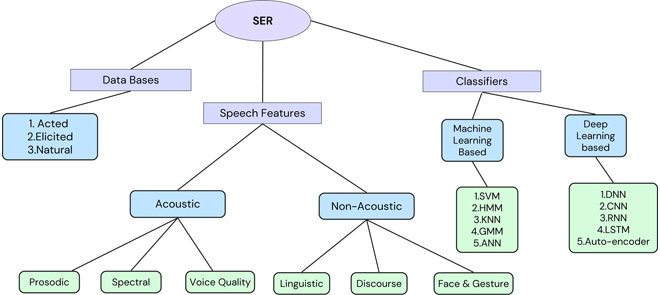
\includegraphics{SER-Overview-Der-Delbabu-2024.png}}
  \caption{Cakupan basis data, fitur, dan \emph{classifier} pada SER}
  \label{fig:2.ser}
  \normalfont Sumber : Dar and Delhibabu (2024)
\end{figure}

Cakupan penerapan SER terus meluas, mulai dari asisten virtual yang
responsif terhadap keadaan pengguna, layanan pelanggan otomatis yang
dapat mendeteksi frustrasi penelepon, hingga sistem pemantauan kesehatan
mental yang menandai perubahan pola emosi dari waktu ke waktu.
Perkembangan representasi \emph{self-supervised} seperti Wav2Vec2 dan
XLSR-53 menjadi salah satu pendorong utama peningkatan akurasi SER
dibandingkan pendekatan fitur \emph{hand-crafted} konvensional.

% ── 2.3 Data Leakage / Group Leakage ──────────────────────────────────
\section{Data Leakage / Group Leakage}
\label{sec:2.3}

Kebocoran data (\emph{data leakage}) (Kapoor and Narayanan, 2023) adalah
kondisi ketika informasi dari data uji secara tidak sengaja ikut
memengaruhi proses pelatihan model, sehingga performa yang terukur pada
data uji tidak lagi mencerminkan kemampuan generalisasi model yang
sesungguhnya pada data baru. Salah satu bentuk kebocoran data yang
sering luput diperhatikan adalah \emph{group leakage}, yaitu kebocoran
yang terjadi ketika beberapa sampel data memiliki keterkaitan atau
berasal dari satu sumber/kelompok yang sama (dikategorikan sebagai
\emph{nonindependence} antara sampel latih dan uji oleh Kapoor and
Narayanan, 2023) -- misalnya beberapa klip ucapan yang berasal dari
rekaman film yang sama -- namun sampel-sampel berkelompok tersebut
tersebar ke sisi latih dan uji sekaligus akibat pembagian data yang
dilakukan secara acak murni terhadap satuan sampel individual (skema
\emph{random}). Ketika hal ini terjadi, model berpotensi mempelajari
ciri-ciri spesifik kelompok tersebut -- misalnya gaya produksi,
karakteristik rekaman, atau suara latar khas suatu film -- sebagai
jalan pintas untuk memprediksi label, alih-alih benar-benar mempelajari
pola yang ingin dikenali (dalam konteks penelitian ini, pola akustik
emosi). Akibatnya, performa yang dilaporkan pada skema \emph{random}
cenderung terlihat lebih tinggi daripada performa sesungguhnya yang
akan diperoleh model pada data dari sumber yang benar-benar baru.

Skema pembagian data \emph{movie-independent} (satu ragam
\emph{grouped split}) mengatasi risiko \emph{group leakage} tersebut
dengan menjaga agar seluruh klip yang berasal dari film yang sama
selalu berada pada sisi \emph{fold} yang sama -- tidak pernah ada satu
film yang klipnya tersebar ke sisi latih dan uji sekaligus. Dengan
demikian, ketika suatu film digunakan sebagai data uji, model
benar-benar belum pernah ``melihat'' karakteristik rekaman film
tersebut selama pelatihan, sehingga performa yang terukur mencerminkan
kemampuan generalisasi model pada sumber rekaman yang genuinely baru.
Preseden penerapan skema \emph{grouped} semacam ini pada SER dilaporkan
oleh Tang et al. (2023), yang menerapkan skema evaluasi
\emph{speaker-independent} -- varian \emph{grouped split} berdasarkan
identitas penutur, bukan berdasarkan film -- untuk mencegah model
mempelajari isyarat spesifik penutur alih-alih pola emosi yang
genuinely general. Penelitian ini menerapkan prinsip yang sama pada
satuan film, karena unit kebocoran yang relevan pada dataset yang
digunakan adalah sumber film, bukan identitas penutur individual.

Penelitian ini membandingkan performa algoritma yang diuji di bawah
kedua skema tersebut -- \emph{random} dan \emph{movie-independent} --
untuk mengukur secara langsung seberapa besar performa yang dilaporkan
berpotensi terinflasi oleh \emph{group leakage} berbasis film, dan
apakah besar inflasi tersebut berbeda antara algoritma berbasis fitur
\emph{hand-crafted} dan algoritma berbasis representasi \emph{self-supervised}.

% ── 2.4 Fitur Hand-Crafted ────────────────────────────────────────────
\section{Fitur Hand-Crafted}
\label{sec:2.4}

Fitur \emph{hand-crafted} adalah representasi sinyal yang diekstraksi
secara manual melalui rangkaian transformasi sinyal yang telah
ditentukan terlebih dahulu (\emph{fixed}) berdasarkan teori dan
pengetahuan domain, alih-alih dipelajari otomatis oleh model dari data.
Pada domain pemrosesan ucapan, fitur \emph{hand-crafted} umumnya
dirancang untuk menangkap karakteristik akustik yang secara teoretis
relevan dengan tugas yang ingin diselesaikan, misalnya intonasi,
energi, nada dasar (\emph{pitch}), atau distribusi frekuensi sinyal.
Karena rangkaian transformasinya sudah ditentukan sejak awal, fitur
\emph{hand-crafted} tidak memerlukan data berlabel maupun proses
pembelajaran untuk diperoleh, berbeda dengan representasi yang
dipelajari model dari data (\emph{learned representations}) yang
parameternya disesuaikan melalui proses pelatihan.

Pendekatan fitur \emph{hand-crafted} banyak digunakan pada penelitian
SER sebelum berkembangnya representasi yang dipelajari model, karena
tidak memerlukan data pra-latih berskala besar dan relatif murah secara
komputasi untuk diekstraksi. Salah satu fitur \emph{hand-crafted} yang
paling umum digunakan pada pemrosesan ucapan adalah Mel-Frequency
Cepstral Coefficients (MFCC), yang digunakan sebagai representasi fitur
\emph{hand-crafted} pada penelitian ini.

% ── 2.5 Mel-Frequency Cepstral Coefficients (MFCC) ───────────────────
\section{Mel-Frequency Cepstral Coefficients (MFCC)}
\label{sec:2.5}

Mel-Frequency Cepstral Coefficients (MFCC) adalah representasi fitur
akustik \emph{hand-crafted} yang secara luas digunakan pada tugas pemrosesan ucapan,
dirancang untuk meniru cara sistem pendengaran manusia mempersepsikan
frekuensi bunyi secara tidak linear (Davis and Mermelstein, 1980).
Alih-alih menggunakan skala frekuensi linear (Hz), MFCC memetakan
spektrum sinyal ke skala mel, yang lebih sensitif terhadap perbedaan
pada frekuensi rendah dibandingkan frekuensi tinggi, sebagaimana
Persamaan \ref{eq:2.mel}.

\begin{equation}
  m = 2595 \log_{10}\left(1 + \frac{f}{700}\right)
  \label{eq:2.mel}
\end{equation}

\noindent
di mana $f$ adalah frekuensi dalam Hz dan $m$ adalah frekuensi
terskala mel yang bersesuaian.

Ekstraksi MFCC dari sinyal ucapan mentah dilakukan melalui serangkaian
tahap sebagaimana digambarkan pada Gambar \ref{fig:2.mfcc}. Sinyal
terlebih dahulu melalui \emph{pre-emphasis} untuk menguatkan komponen
frekuensi tinggi, kemudian dibagi menjadi bingkai-bingkai pendek
(\emph{framing}) yang tumpang tindih dan dikalikan fungsi jendela
(\emph{windowing}) untuk mengurangi efek diskontinuitas di tepi bingkai.
Setiap bingkai kemudian ditransformasi ke domain frekuensi menggunakan
\emph{Fast Fourier Transform} (FFT) untuk memperoleh spektrum daya, yang
selanjutnya difilter menggunakan sekumpulan filter \emph{bank} berskala
mel (Persamaan \ref{eq:2.mel}) untuk memperoleh energi pada tiap pita
frekuensi mel. Energi tersebut diambil logaritmanya untuk mendekati
persepsi kenyaringan manusia yang bersifat logaritmik, kemudian
ditransformasi menggunakan \emph{Discrete Cosine Transform} (DCT) untuk
mendekorelasi energi antarpita dan menghasilkan koefisien cepstral
akhir.

\begin{figure}[H]
  \centering
  \gambarbesar{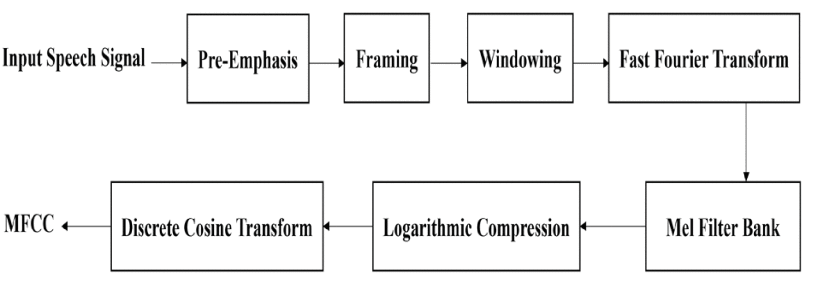
\includegraphics{MFCC-Block-DIagram.png}}
  \caption{Pipeline ekstraksi Mel-Frequency Cepstral Coefficients (MFCC)}
  \label{fig:2.mfcc}
  \normalfont Sumber : Alashban and Alotaibi (2023)
\end{figure}

Berbeda dengan representasi yang dipelajari model dari data
(\emph{learned representations}), MFCC dihitung langsung dari sinyal
melalui rangkaian transformasi sinyal yang telah ditentukan
(\emph{fixed}), tanpa proses pembelajaran. Karakteristik inilah yang
mendasari penggunaan MFCC sebagai fitur \emph{hand-crafted} pada
algoritma \emph{baseline} dalam penelitian ini.

% ── 2.6 Convolutional Neural Network (CNN) ───────────────────────────
\section{Convolutional Neural Network (CNN)}
\label{sec:2.6}

\emph{Convolutional neural network} (CNN) adalah arsitektur jaringan
saraf tiruan yang dirancang untuk memproses data yang memiliki struktur
grid, seperti citra dua dimensi atau spektrogram ucapan, dengan
memanfaatkan operasi konvolusi untuk mengekstraksi pola-pola lokal
secara bertingkat (LeCun et al., 1998). Arsitektur CNN umumnya terdiri
atas tiga jenis lapisan utama, sebagaimana digambarkan pada Gambar
\ref{fig:2.cnn}: (1) lapisan konvolusi (\emph{convolutional layer}),
yang menerapkan sejumlah filter/\emph{kernel} berukuran kecil secara
bergeser di sepanjang data masukan untuk mendeteksi pola lokal seperti
tepi atau tekstur pada tahap awal, dan pola yang lebih kompleks pada
lapisan berikutnya; (2) lapisan \emph{pooling}, yang mereduksi dimensi
spasial representasi sambil mempertahankan informasi penting, sehingga
jaringan lebih tahan terhadap pergeseran kecil pada data masukan dan
lebih efisien secara komputasi; dan (3) lapisan terhubung penuh
(\emph{fully-connected layer}), yang menggabungkan seluruh fitur yang
telah diekstraksi untuk menghasilkan keluaran akhir, misalnya
probabilitas kelas pada tugas klasifikasi. Secara garis besar, lapisan
konvolusi dan \emph{pooling} membentuk tahap ekstraksi fitur
(\emph{feature extraction}), sedangkan lapisan terhubung penuh membentuk
tahap klasifikasi (\emph{classification}), sebagaimana ditunjukkan pada
Gambar \ref{fig:2.cnn}.

\begin{figure}[H]
  \centering
  \gambarbesar{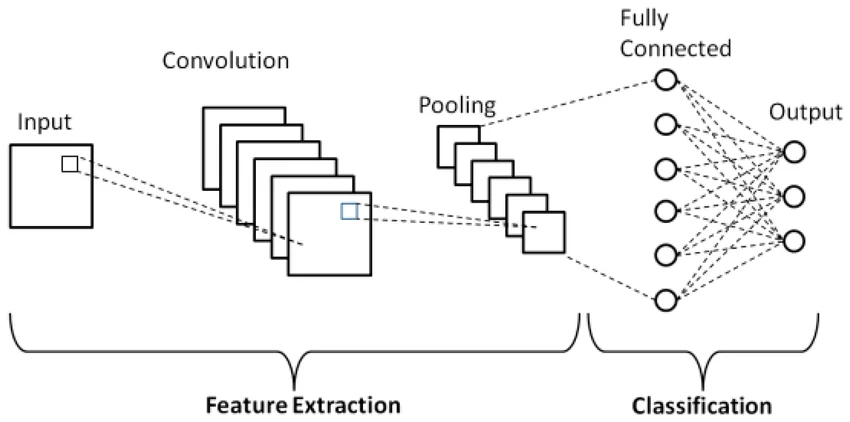
\includegraphics{Basic-CNN-Diagram.png}}
  \caption{Arsitektur umum Convolutional Neural Network (CNN)}
  \label{fig:2.cnn}
  \normalfont Sumber : Phung and Rhee (2019)
\end{figure}

Kemampuan lapisan konvolusi mendeteksi pola lokal menjadikan CNN cocok
untuk memproses fitur MFCC, yang berbentuk grid dua dimensi berupa
koefisien cepstral pada sumbu vertikal dan bingkai waktu pada sumbu
horizontal -- pola akustik emosi yang relevan seringkali muncul sebagai
struktur lokal pada grid tersebut, misalnya perubahan energi pada
rentang waktu dan pita frekuensi tertentu. Karakteristik inilah yang
mendasari penggunaan CNN sebagai \emph{classifier} pada algoritma
\emph{baseline} dalam penelitian ini, mengikuti pendekatan yang sudah
banyak digunakan pada penelitian SER berbasis fitur \emph{hand-crafted}.

% ── 2.7 Pembelajaran Self-Supervised ─────────────────────────────────
\section{Pembelajaran Self-Supervised}
\label{sec:2.7}

Pembelajaran \emph{self-supervised} adalah paradigma pembelajaran mesin
yang melatih model pada data tanpa label dengan cara menciptakan sinyal
pengawasan (\emph{supervision signal}) dari data itu sendiri, alih-alih
memerlukan label yang dianotasi manusia (Liu et al., 2023). Model
dilatih untuk menyelesaikan \emph{pretext task}, yaitu tugas bantu yang
dirancang agar penyelesaiannya mengharuskan model mempelajari struktur
dan pola yang mendasari data, misalnya memprediksi bagian data yang
disembunyikan dari bagian yang tersisa. Sebagaimana ditunjukkan pada
Gambar \ref{fig:2.ssl}, bobot \emph{encoder} yang telah dilatih pada
\emph{pretext task} menggunakan data tanpa label kemudian ditransfer
(\emph{transfer weights}) sebagai titik awal model pada tugas hilir
(\emph{downstream task}) yang sesungguhnya, sebelum diadaptasi lebih
lanjut (\emph{fine-tuned}) menggunakan data berlabel, seperti
klasifikasi emosi pada penelitian ini.

\begin{figure}[H]
  \centering
  \gambarbesar{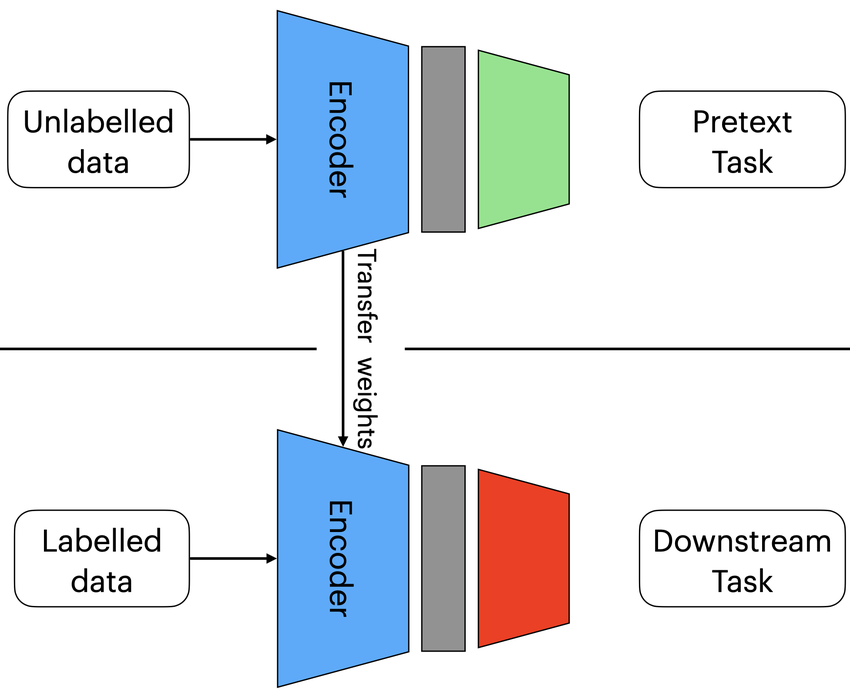
\includegraphics{Self-Supervised-Diagram.png}}
  \caption{Alur umum pembelajaran Self-Supervised}
  \label{fig:2.ssl}
  \normalfont Sumber : Del Pup and Atzori (2023)
\end{figure}

Keunggulan utama paradigma ini adalah kemampuannya memanfaatkan data
tanpa label dalam jumlah besar, yang jauh lebih mudah dan murah diperoleh
dibandingkan data berlabel. Karakteristik inilah yang mendasari
penggunaannya secara luas pada domain ucapan, termasuk pada backbone
Wav2Vec2 dan XLSR-53 yang digunakan dalam penelitian ini.

% ── 2.8 Wav2Vec2 ──────────────────────────────────────────────────────
\section{Wav2Vec2}
\label{sec:2.8}

Wav2Vec2 adalah arsitektur pembelajaran \emph{self-supervised} untuk
representasi ucapan yang dilatih pada volume data ucapan tanpa label
berskala besar (Baevski et al., 2020). Arsitekturnya terdiri atas tiga
komponen utama, sebagaimana digambarkan pada Gambar \ref{fig:2.wav2vec2}:
(1) \emph{feature encoder} berbasis \emph{convolutional neural network}
(CNN) yang mengubah gelombang ucapan mentah menjadi representasi laten
$Z$ pada resolusi waktu yang lebih rendah; (2) \emph{context network}
berbasis Transformer yang mengolah $Z$ (dengan sebagian di antaranya
disembunyikan/\emph{masked}) menjadi representasi terkontekstualisasi
$C$; dan (3) modul kuantisasi yang mendiskretkan $Z$ menjadi target
kuantisasi $Q$, khusus digunakan pada tahap pra-latih untuk menghitung
\emph{contrastive loss} yang mendorong model membedakan representasi
kuantisasi yang benar dari sejumlah pengganggu (\emph{distractors}).

\begin{figure}[H]
  \centering
  \gambarbesar{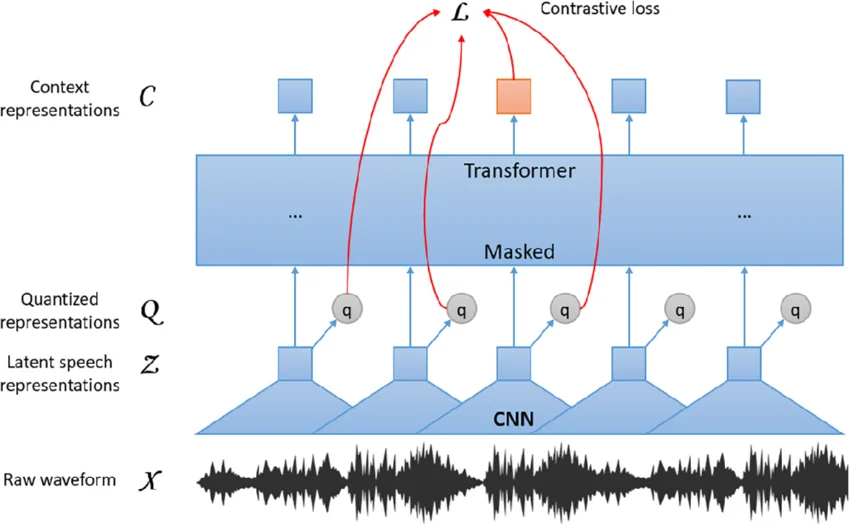
\includegraphics{WAV2VEC2-Diagram.png}}
  \caption{Arsitektur Wav2Vec2}
  \label{fig:2.wav2vec2}
  \normalfont Sumber : Ovalle et al. (2024)
\end{figure}

Representasi $C$ yang dihasilkan oleh \emph{context network} inilah yang
menjadi keluaran utama Wav2Vec2 untuk dimanfaatkan pada tugas hilir
(\emph{downstream task}), termasuk SER pada penelitian ini.

% ── 2.9 XLSR-53 ───────────────────────────────────────────────────────
\section{XLSR-53}
\label{sec:2.9}

XLSR merupakan varian multibahasa dari Wav2Vec2 yang dilatih pada data
ucapan tanpa label dari banyak bahasa sekaligus, menggunakan arsitektur
dan tujuan pra-latih yang sama, namun dengan korpus pra-latih gabungan
lintas bahasa (Conneau et al., 2021). Karena dilatih lintas bahasa,
representasi yang dihasilkan XLSR cenderung menangkap struktur akustik
yang lebih umum dan dapat menggeneralisasi lintas bahasa dibandingkan
model yang hanya dilatih pada satu bahasa saja. XLSR-53 adalah varian
XLSR yang dilatih pada korpus gabungan dari 53 bahasa. Karakteristik
inilah yang mendasari pemilihan XLSR-53 sebagai backbone algoritma SOTA
dalam penelitian ini: bobot dasar backbone tetap dibekukan
(\emph{frozen}), namun diberi matriks adaptasi tambahan berperingkat
rendah (LoRA) yang dilatih untuk menyesuaikan representasi ke tugas
SER, alih-alih memperbarui seluruh parameter backbone secara langsung.

% ── 2.10 Low-Rank Adaptation (LoRA) ──────────────────────────────────
\section{Low-Rank Adaptation (LoRA)}
\label{sec:2.10}

\emph{Low-Rank Adaptation} (LoRA) adalah strategi \emph{fine-tuning}
efisien-parameter yang membekukan seluruh bobot model dasar $W_0$ dan
hanya melatih sepasang matriks tambahan berperingkat rendah
(\emph{low-rank}) yang disisipkan secara paralel (Hu et al., 2022).
Untuk suatu lapisan dengan bobot pra-latih $W_0 \in \mathbb{R}^{d \times
k}$, LoRA merepresentasikan pembaruan bobot $\Delta W$ sebagai perkalian
dua matriks berperingkat rendah $B \in \mathbb{R}^{d \times r}$ dan $A
\in \mathbb{R}^{r \times k}$, dengan $r \ll \min(d, k)$, sehingga keluaran
lapisan tersebut untuk masukan $x$ dihitung sebagaimana Persamaan
\ref{eq:2.lora}.

\begin{equation}
  h = W_0 x + \Delta W x = W_0 x + BA x
  \label{eq:2.lora}
\end{equation}

\noindent
Gambar \ref{fig:2.lora} membandingkan skema tersebut dengan \emph{full
fine-tuning} konvensional. Pada \emph{full fine-tuning} (kiri),
pembaruan bobot $\Delta W$ dilatih penuh sebagai satu matriks padat
berukuran sama dengan $W_0$. Pada LoRA (kanan), bobot dasar $W_0$
dibekukan (ditandai ikon salju) sementara hanya matriks $A$ dan $B$
berperingkat rendah yang dilatih (ditandai ikon api), sebelum hasil
keduanya dijumlahkan menjadi keluaran $h$.

\begin{figure}[H]
  \centering
  \gambarbesar{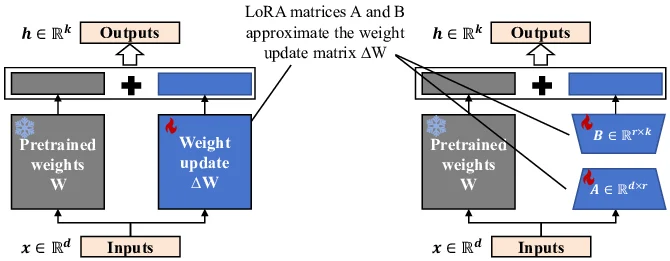
\includegraphics{Regular-Fine-TUne-VS-LoRA-diagram-.png}}
  \caption{Perbandingan full fine-tuning dan LoRA}
  \label{fig:2.lora}
  \normalfont Sumber : Lu et al. (2024)
\end{figure}

Karena jumlah parameter pada $A$ dan $B$ jauh lebih sedikit daripada
jumlah parameter $W_0$, LoRA menawarkan efisiensi komputasi dan memori
yang signifikan dibandingkan \emph{full fine-tuning}, yang memperbarui
seluruh parameter $W_0$ secara langsung. Efisiensi ini relevan bagi
penelitian dengan keterbatasan sumber daya komputasi. Efektivitas LoRA
pada arsitektur berbasis Wav2Vec2 secara spesifik telah dibuktikan pada
tugas deteksi audio sintetis, di mana LoRA mencapai performa setara
dengan \emph{full fine-tuning} sekaligus mengurangi jumlah parameter
yang dilatih hingga 198 kali lipat (Wang et al., 2023). Pada tugas SER
secara lebih spesifik, kombinasi LoRA dengan metode
\emph{parameter-efficient fine-tuning} lainnya terbukti melampaui
performa \emph{full fine-tuning} pada backbone Wav2Vec2 dan HuBERT,
sekaligus hanya melatih sekitar 2--3\% dari total parameter
(Lashkarashvili et al., 2024). Karakteristik inilah yang mendasari
penggunaan LoRA untuk mengadaptasi backbone XLSR-53 pada algoritma SOTA
dalam penelitian ini, alih-alih memperbarui seluruh parameter backbone
secara langsung.

% ── 2.11 Evaluasi Model ──────────────────────────────────────────────
\section{Evaluasi Model}
\label{sec:2.11}

Akurasi, presisi, recall, dan F1-score adalah empat metrik yang umum
digunakan untuk mengevaluasi performa model klasifikasi (Powers, 2011).
Akurasi mengukur proporsi prediksi yang benar terhadap keseluruhan data
uji, sehingga memberikan gambaran umum performa model, sebagaimana
Persamaan \ref{eq:2.akurasi}.

\begin{equation}
  \text{Akurasi} = \frac{TP + TN}{TP + TN + FP + FN}
  \label{eq:2.akurasi}
\end{equation}

\noindent
di mana $TP$ = \emph{True Positive}, $TN$ = \emph{True Negative}, $FP$ =
\emph{False Positive}, $FN$ = \emph{False Negative}.

Akan tetapi, pada data dengan sebaran kelas yang tidak seimbang, akurasi
dapat memberikan gambaran yang menyesatkan, karena model yang selalu
memprediksi kelas mayoritas tetap dapat memperoleh akurasi tinggi tanpa
benar-benar mengenali kelas minoritas. Presisi mengukur proporsi
prediksi positif yang benar-benar tepat, sebagaimana Persamaan
\ref{eq:2.presisi}.

\begin{equation}
  \text{Presisi} = \frac{TP}{TP + FP}
  \label{eq:2.presisi}
\end{equation}

\noindent
Recall mengukur proporsi kasus positif yang berhasil dikenali model,
sebagaimana Persamaan \ref{eq:2.recall}.

\begin{equation}
  \text{Recall} = \frac{TP}{TP + FN}
  \label{eq:2.recall}
\end{equation}

\noindent
Presisi dan recall sering kali saling bertukar (\emph{trade-off}):
menaikkan salah satu cenderung menurunkan yang lain. F1-score mengatasi
keterbatasan ini dengan merepresentasikan rata-rata harmonis keduanya,
sebagaimana Persamaan \ref{eq:2.f1}.

\begin{equation}
  F_1 = 2 \cdot \frac{\text{Presisi} \times \text{Recall}}{\text{Presisi} + \text{Recall}}
  \label{eq:2.f1}
\end{equation}

Keempat metrik ini digunakan bersama dalam penelitian ini untuk
memberikan gambaran performa yang lebih menyeluruh terhadap setiap
kondisi yang dibandingkan. Meskipun skema kelas emosi pada dataset yang
digunakan dalam penelitian ini seimbang antarkelas, akurasi saja tidak
menunjukkan pola kesalahan per kelas, sedangkan presisi, recall, dan
F1-score memberikan gambaran lebih rinci mengenai kelas emosi mana yang
lebih sering tertukar atau lebih sulit dikenali model.

% ── 2.12 Validasi Silang K-Fold ───────────────────────────────────────
\section{Validasi Silang K-Fold}
\label{sec:2.12}

Validasi silang k-fold adalah teknik evaluasi yang membagi data menjadi
$k$ bagian (\emph{fold}) berukuran relatif sama, dengan setiap bagian
secara bergantian digunakan sebagai data uji sementara $k-1$ bagian
lainnya digunakan sebagai data latih, sehingga setiap bagian data pernah
menjadi data uji tepat satu kali (Kohavi, 1995). Gambar
\ref{fig:2.kfold} mengilustrasikan mekanisme umum tersebut: \emph{fold}
uji (biru) berpindah bergiliran pada tiap iterasi sementara \emph{fold}
sisanya berperan sebagai data latih, dengan hasil evaluasi $E_i$ dari
tiap iterasi dirata-ratakan menjadi estimasi performa akhir $E$.
Penelitian ini secara spesifik menggunakan $k=6$.

\begin{figure}[H]
  \centering
  \gambarbesar{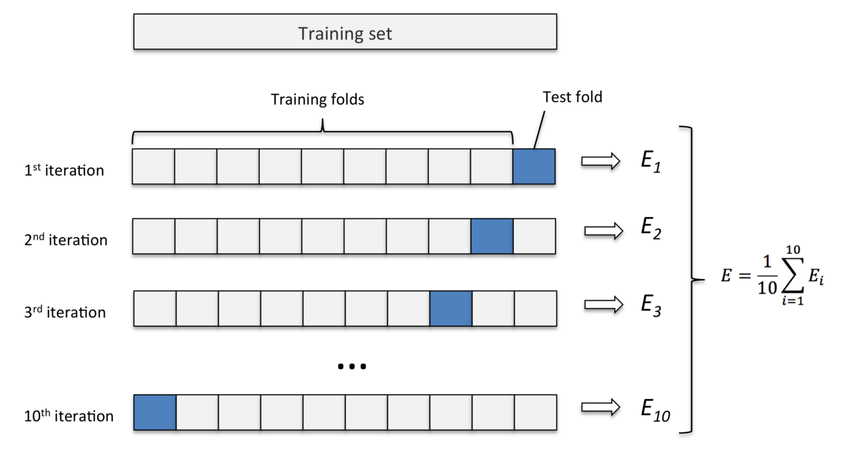
\includegraphics{K-Fold-Diagram.png}}
  \caption{Ilustrasi mekanisme validasi silang k-fold}
  \label{fig:2.kfold}
  \normalfont Sumber : Ashfaque and Iqbal (2019)
\end{figure}

Teknik ini menghasilkan $k$ observasi akurasi dan F1-score, satu untuk
setiap fold, sehingga memungkinkan pengujian konsistensi performa
antar-fold untuk setiap kondisi yang diuji, bukan hanya satu nilai
tunggal dari satu kali pengujian.

% ── 2.13 Pengujian Signifikansi Statistik ────────────────────────────
\section{Pengujian Signifikansi Statistik}
\label{sec:2.13}

Untuk menguji apakah perbedaan performa antarkondisi hasil validasi
silang k-fold bersifat signifikan secara statistik, $k$ observasi yang
diperoleh terlebih dahulu diuji normalitasnya menggunakan uji
Shapiro-Wilk, yang menghitung statistik $W$ sebagaimana Persamaan
\ref{eq:2.shapirowilk} (Shapiro and Wilk, 1965).

\begin{equation}
  W = \frac{\left(\sum_{i=1}^{n} a_i x_{(i)}\right)^2}{\sum_{i=1}^{n} (x_i - \bar{x})^2}
  \label{eq:2.shapirowilk}
\end{equation}

\noindent
di mana $x_{(i)}$ adalah nilai observasi ke-$i$ setelah diurutkan
menaik (statistik urutan), $\bar{x}$ adalah rata-rata observasi, $n$
adalah jumlah observasi (jumlah fold), dan $a_i$ adalah konstanta yang
diturunkan dari rata-rata, ragam, dan kovarians statistik urutan sampel
berdistribusi normal berukuran $n$. Nilai $W$ yang mendekati 1
mengindikasikan data mendekati distribusi normal.

Apabila data berdistribusi normal, pengujian dilanjutkan dengan
\emph{paired t-test}, yang menghitung statistik uji $t$ dari selisih
berpasangan $d_i$ antara dua kondisi pada fold yang sama, sebagaimana
Persamaan \ref{eq:2.ttest}.

\begin{equation}
  t = \frac{\bar{d}}{s_d / \sqrt{n}}
  \label{eq:2.ttest}
\end{equation}

\noindent
di mana $\bar{d}$ adalah rata-rata selisih berpasangan, $s_d$ adalah
simpangan baku selisih tersebut, dan $n$ adalah jumlah fold. Apabila
data tidak berdistribusi normal, digunakan \emph{Wilcoxon signed-rank
test} sebagai alternatif non-parametrik yang tidak mengasumsikan
distribusi tertentu, dengan statistik uji $W$ sebagaimana Persamaan
\ref{eq:2.wilcoxon} (Wilcoxon, 1945).

\begin{equation}
  W = \sum_{i=1}^{n} \operatorname{sgn}(d_i) \, R_i
  \label{eq:2.wilcoxon}
\end{equation}

\noindent
di mana $d_i$ adalah selisih berpasangan pada fold ke-$i$, $R_i$ adalah
peringkat (\emph{rank}) dari $|d_i|$ di antara seluruh selisih mutlak
$|d_1|, \dots, |d_n|$, dan $\operatorname{sgn}(d_i)$ bernilai $+1$
apabila $d_i>0$ dan $-1$ apabila $d_i<0$.

% =====================================================================
%  BAB 3 — METODOLOGI PENELITIAN
% =====================================================================

\chapter{Metodologi Penelitian}

\section{Tipe Penelitian}
\label{sec:3.1}

Penelitian ini merupakan penelitian non-implementatif analitik dengan
pendekatan kuantitatif, karena berfokus pada analisis pengaruh strategi
\emph{fine-tuning} terhadap akurasi klasifikasi emosi ucapan, bukan pada
pengembangan sistem atau perangkat lunak siap pakai. Sifat analitik
ditunjukkan melalui pengolahan data hasil observasi akurasi dan F1-score
dari setiap strategi \emph{fine-tuning} untuk mengkaji hubungan antara
strategi yang diterapkan dan performa klasifikasi emosi yang dihasilkan.
Pendekatan kuantitatif digunakan karena data berupa nilai numerik hasil
evaluasi model yang dianalisis menggunakan metrik akurasi, F1-score, dan
pengujian signifikansi statistik. Model-model yang di-\emph{fine-tune}
pada penelitian ini berfungsi sebagai instrumen untuk menghasilkan data
observasi tersebut, bukan sebagai produk/artefak utama penelitian.

\begin{figure}[H]
  \centering
  \begin{tikzpicture}[node distance=8mm]
    \node[term] (mulai)   {Mulai};
    \node[proc] (studi)   [below=of mulai]    {Studi Literatur};
    \node[proc] (data)    [below=of studi]    {Pengumpulan Data};
    \node[proc] (sumber)  [below=of data]     {Fine-Tuning Sumber};
    \node[proc] (target)  [below=of sumber]   {Fine-Tuning Target};
    \node[proc] (evaluasi)[below=of target]   {Evaluasi K-Fold};
    \node[proc] (kinerja) [below=of evaluasi] {Analisis Kinerja Komputasi};
    \node[proc] (analisis)[below=of kinerja]  {Analisis Hasil};
    \node[term] (selesai) [below=of analisis] {Selesai};

    \draw[arr] (mulai)    -- (studi);
    \draw[arr] (studi)    -- (data);
    \draw[arr] (data)     -- (sumber);
    \draw[arr] (sumber)   -- (target);
    \draw[arr] (target)   -- (evaluasi);
    \draw[arr] (evaluasi) -- (kinerja);
    \draw[arr] (kinerja)  -- (analisis);
    \draw[arr] (analisis) -- (selesai);
  \end{tikzpicture}
  \caption{Diagram alir metode penelitian}
  \label{fig:3.alur}
\end{figure}

Diagram alir metode penelitian ini ditunjukkan pada Gambar
\ref{fig:3.alur}. Tahap awal penelitian diawali dengan studi literatur,
yang bertujuan untuk mengkaji teori, metode, serta penelitian terdahulu
yang relevan dengan SER, pembelajaran \emph{self-supervised}, dan
\emph{cross-lingual transfer}. Tahap berikutnya adalah pengumpulan data,
yaitu proses pengumpulan korpus emosi berbahasa Inggris sebagai sumber
dan dataset SER berbahasa Indonesia sebagai target. Data yang telah
diperoleh selanjutnya diproses pada tahap \emph{fine-tuning} sumber
untuk melatih backbone \emph{self-supervised} mengenali pola akustik
emosi secara umum. Setelah itu dilakukan \emph{fine-tuning} target untuk
mengadaptasi model dasar ke data Indonesia melalui beberapa skema
strategi. Tahap berikutnya adalah evaluasi k-fold untuk menilai performa
setiap strategi menggunakan skema validasi silang dan pengujian
signifikansi statistik, dilanjutkan analisis kinerja komputasi untuk
membandingkan waktu pelatihan dan penggunaan memori antarkondisi. Hasil
kedua evaluasi tersebut kemudian digunakan sebagai dasar pada tahap
analisis hasil, yang merangkum temuan penelitian serta menjawab rumusan
masalah yang telah dipaparkan.

\section{Studi Literatur}
\label{sec:3.2}

Studi literatur merupakan tahap awal penelitian yang bertujuan untuk
mempelajari dan memahami teori, konsep, serta hasil penelitian terdahulu
yang berkaitan dengan SER, pembelajaran \emph{self-supervised},
representasi Wav2Vec2/XLSR, dan \emph{cross-lingual transfer}. Pada
tahap ini dilakukan pengkajian terhadap jurnal, prosiding konferensi,
dan sumber ilmiah relevan untuk memastikan celah penelitian pada Bab 2
Landasan Kepustakaan belum terjawab oleh penelitian lain, sekaligus
menentukan backbone model dan skema \emph{fine-tuning} yang sesuai
dengan tujuan penelitian.

\section{Pengumpulan Data}
\label{sec:3.3}

Tahap ini mengumpulkan dua kelompok data, yaitu korpus emosi berbahasa
Inggris sebagai sumber pada tahap \emph{fine-tuning} pertama
(RAVDESS/CREMA-D), dan dataset E-SERAVD (Santoso, Budianto and Dutono,
2026) sebagai target berbahasa Indonesia pada tahap \emph{fine-tuning}
kedua. Skema kelas emosi pada korpus sumber disesuaikan dengan skema
empat kelas yang tersedia pada E-SERAVD (marah, senang, netral, sedih),
sehingga perbandingan antarstrategi \emph{fine-tuning} dapat dilakukan
secara adil.

Karakteristik masing-masing korpus dijelaskan sebagai berikut. RAVDESS
adalah korpus ucapan emosional berbahasa Inggris yang direkam oleh 24
aktor profesional (12 perempuan, 12 laki-laki), mencakup 8 kategori
emosi (netral, tenang, senang, sedih, marah, takut, jijik, dan terkejut)
(Livingstone and Russo, 2018). CREMA-D adalah korpus ucapan emosional
berbahasa Inggris yang direkam oleh 91 aktor dengan latar belakang usia
dan etnis yang beragam, mencakup 6 kategori emosi (marah, jijik, takut,
senang, netral, dan sedih) (Cao et al., 2014). Kedua korpus ini dipilih
sebagai sumber karena tersedia secara publik, telah banyak digunakan
pada penelitian SER sebelumnya, dan mencakup kategori emosi yang secara
umum beririsan dengan skema kelas pada dataset target. Tabel
\ref{tab:3.dataset} merangkum karakteristik ketiga dataset yang
digunakan.

\begin{table}[H]
  \centering
  \caption{Karakteristik dataset yang digunakan}
  \label{tab:3.dataset}
  \begin{adjustbox}{max width=\textwidth}
  \begin{tabular}{p{3.8cm} l l p{2.6cm} p{1.8cm}}
    \toprule
    \textbf{Dataset} & \textbf{Peran} & \textbf{Bahasa} & \textbf{Jumlah Sampel} & \textbf{Jumlah Kelas} \\
    \midrule
    RAVDESS & Sumber & Inggris & 1.440 & 8 \\
    CREMA-D & Sumber & Inggris & 7.442 & 6 \\
    E-SERAVD & Target & Indonesia & $\sim$5.049 & 4 \\
    \bottomrule
  \end{tabular}
  \end{adjustbox}
\end{table}

\noindent
Jumlah sampel untuk RAVDESS dan CREMA-D di atas mengacu pada dokumentasi
resmi masing-masing korpus. E-SERAVD memiliki sekitar 5.049 sampel
dengan distribusi 1.202 marah, 1.228 senang, 2.075 netral, dan 899 sedih
(Santoso, Budianto and Dutono, 2026); angka ini masih perlu diverifikasi
ulang terhadap dokumentasi resmi dataset sebelum benar-benar diperoleh.
Dataset SER Indonesia lain seperti IndoWaveSentiment (Nugroho et al.,
2025) tidak digunakan sebagai target pada penelitian ini karena skala
dan skema kelasnya berbeda dari E-SERAVD, namun disebutkan kembali
sebagai arah pengembangan pada Bab 6.

\section{Fine-Tuning Sumber}
\label{sec:3.4}

Backbone yang digunakan adalah model dasar XLSR-53
(\path{facebook/wav2vec2-large-xlsr-53}) tanpa \emph{fine-tuning}
tambahan dari pihak lain untuk Bahasa Indonesia -- berbeda dari
pendekatan Nugroho et al. (2025) yang menguji model dasar XLSR-Wav2Vec2
yang sudah di-\emph{fine-tune} untuk ucapan Indonesia (lihat Subbab
\ref{sec:2.4}). Pemilihan ini disengaja: dengan titik awal yang identik
di keempat kondisi eksperimen (Subbab \ref{sec:3.5}), perbedaan performa
yang teramati dapat ditarik ke strategi \emph{fine-tuning} yang diuji
dalam penelitian ini, bukan tercampur dengan efek \emph{fine-tuning}
pihak lain yang sudah menempel pada checkpoint.

Tahap ini melatih backbone \emph{self-supervised} (Wav2Vec2/XLSR-53)
pada korpus emosi berbahasa Inggris agar model mampu mengenali pola
akustik emosi secara umum, menghasilkan model dasar yang selanjutnya
akan diadaptasi ke data target pada tahap berikutnya. Tahap ini
dijalankan sekali saja; bobot hasilnya dipakai ulang sebagai titik awal
untuk semua fold pada Kondisi C dan D (Subbab \ref{sec:3.5}), bukan
diulang per-fold, karena \emph{fine-tuning} tahap sumber tidak
bergantung pada pembagian fold data target.

\section{Fine-Tuning Target}
\label{sec:3.5}

Tahap ini mengadaptasi model ke data Indonesia melalui dua axis desain
yang independen: (1) \emph{stage}, yaitu apakah model melalui
\emph{fine-tuning} dua tahap atau langsung dilatih pada data target
(\emph{single-stage}); dan (2) metode adaptasi, yaitu \emph{full
fine-tuning} yang memperbarui seluruh parameter model, atau LoRA yang
hanya memperbarui parameter tambahan berjumlah kecil. Kombinasi kedua
axis tersebut menghasilkan empat kondisi eksperimen sebagaimana
dirangkum pada Tabel \ref{tab:3.kondisi}.

\begin{table}[H]
  \centering
  \caption{Empat kondisi eksperimen (desain 2$\times$2)}
  \label{tab:3.kondisi}
  \begin{tabular}{c l l}
    \toprule
    \textbf{Kondisi} & \textbf{Stage} & \textbf{Metode Adaptasi} \\
    \midrule
    A & Single-stage & Full Fine-Tuning \\
    B & Single-stage & LoRA \\
    C & Two-stage    & Full Fine-Tuning \\
    D & Two-stage    & LoRA \\
    \bottomrule
  \end{tabular}
\end{table}

\noindent
Backbone yang digunakan sama persis (XLSR-53, Subbab \ref{sec:3.4}) di
keempat kondisi -- yang berbeda hanya resep \emph{fine-tuning}-nya --
supaya perbedaan hasil antarkondisi dapat ditarik ke strategi
\emph{fine-tuning} yang diuji, bukan ke perbedaan arsitektur atau titik
awal model. Kondisi A dan B tidak melalui tahap \emph{fine-tuning}
sumber (Subbab \ref{sec:3.4}) dan langsung dilatih pada data target,
sedangkan Kondisi C dan D memakai bobot hasil \emph{fine-tuning} sumber
sebagai titik awal. Validasi silang k-fold (Subbab \ref{sec:3.6})
diterapkan pada level adaptasi target ini untuk keempat kondisi. Sebagai
mitigasi risiko, direkomendasikan menjalankan \emph{pilot run} (1
kondisi $\times$ 1 fold) pada perangkat keras sebenarnya sebelum
menjalankan grid eksperimen penuh, untuk memverifikasi estimasi waktu
dan VRAM pada Subbab \ref{sec:3.10.2} dengan data riil.

\section{Evaluasi K-Fold}
\label{sec:3.6}

Tahap ini mengevaluasi setiap kondisi eksperimen menggunakan skema
validasi silang k-fold, sehingga diperoleh beberapa observasi akurasi
dan F1-score per fold untuk masing-masing kondisi. Data hasil observasi
tersebut kemudian diuji normalitasnya menggunakan uji Shapiro-Wilk. Jika
data berdistribusi normal, pengujian dilanjutkan dengan \emph{paired
t-test}; jika tidak, digunakan \emph{Wilcoxon signed-rank test}.
Pengujian ini bertujuan untuk mengetahui signifikansi statistik
perbedaan performa antarkondisi, menjawab hipotesis yang telah
dirumuskan pada Subbab 1.3.

\section{Analisis Kinerja Komputasi}
\label{sec:3.7}

Tahap ini menganalisis kinerja komputasi setiap kondisi eksperimen
(Kondisi A--D), meliputi waktu pelatihan dan penggunaan memori (VRAM)
sebagaimana didefinisikan pada Subbab \ref{sec:2.9.2}. Waktu pelatihan
dicatat dari awal hingga akhir proses pelatihan pada tiap fold untuk
tahap \emph{fine-tuning} target (Subbab \ref{sec:3.5}); durasi
\emph{fine-tuning} sumber (Subbab \ref{sec:3.4}) dicatat terpisah karena
hanya dijalankan sekali dan dipakai bersama oleh Kondisi C dan D.
Penggunaan memori diukur sebagai puncak alokasi VRAM selama pelatihan
pada tiap kondisi. Secara teknis, waktu pelatihan dicatat menggunakan
\texttt{time.perf\_counter()}, sedangkan puncak penggunaan VRAM dicatat
menggunakan \texttt{torch.cuda.max\_memory\_allocated()} setelah
\texttt{reset\_peak\_memory\_stats()} dipanggil di awal tiap fold. Kedua
metrik ini dibandingkan secara deskriptif
antarkondisi, dengan perhatian khusus pada perbandingan Kondisi A vs B
dan Kondisi C vs D (axis \emph{full fine-tuning} vs LoRA) untuk menjawab
Rumusan Masalah 2 dari sisi efisiensi, melengkapi pengujian signifikansi
statistik akurasi dan F1-score pada Subbab \ref{sec:3.6}.

\section{Analisis Hasil}
\label{sec:3.8}

Tahap ini menafsirkan hasil pengujian signifikansi statistik dan
analisis kinerja komputasi untuk menjawab rumusan masalah penelitian,
serta menyusun rekomendasi strategi \emph{fine-tuning} yang paling
sesuai untuk pengembangan SER berbahasa Indonesia berdasarkan temuan
yang diperoleh.

\section{Kesimpulan dan Saran}
\label{sec:3.9}

Penarikan kesimpulan dilaksanakan setelah seluruh tahap evaluasi dan
analisis hasil selesai. Kesimpulan memuat jawaban atas rumusan masalah
yang telah dituliskan sebelumnya, mengacu pada hasil pengujian
signifikansi statistik dari setiap strategi \emph{fine-tuning} yang
dibandingkan. Selain kesimpulan, disusun pula saran sebagai bahan
pertimbangan dan perbaikan untuk penelitian selanjutnya, misalnya
perluasan cakupan korpus sumber atau backbone model yang diuji.

\section{Peralatan Pendukung}
\label{sec:3.10}

Peralatan pendukung yang digunakan dalam penelitian ini terdiri atas
perangkat lunak (\emph{software}) dan perangkat keras (\emph{hardware}).

\subsection{Perangkat Lunak (Software)}
\label{sec:3.10.1}

Perangkat lunak yang digunakan dalam mendukung penelitian ini sebagai
berikut.

\begin{enumerate}
  \item Bahasa pemrograman Python.
  \item Kerangka kerja \emph{deep learning} untuk pelatihan dan
        \emph{fine-tuning} model Wav2Vec2/XLSR.
  \item Pustaka untuk implementasi LoRA.
  \item Pustaka optimizer 8-bit (\texttt{bitsandbytes}) untuk mitigasi
        VRAM pada kondisi \emph{full fine-tuning}.
  \item Pustaka statistik untuk pengujian normalitas dan uji
        signifikansi.
  \item GitHub untuk pengelolaan versi kode sumber dan eksperimen.
\end{enumerate}

\subsection{Perangkat Keras (Hardware)}
\label{sec:3.10.2}

Perangkat keras yang digunakan dalam mendukung penelitian ini sebagai
berikut.

\begin{enumerate}
  \item 2 unit GPU NVIDIA GeForce RTX 3060 6GB (server lab, dipinjamkan).
  \item RAM dan penyimpanan: [\emph{diisi sesuai spesifikasi server lab
        yang sebenarnya dipakai}].
\end{enumerate}

Kecukupan VRAM \emph{per kartu} dianalisis terhadap ukuran backbone
(sekitar 317 juta parameter), sebagaimana dirangkum pada Tabel
\ref{tab:3.vram}.

\begin{table}[H]
  \centering
  \caption{Estimasi kecukupan VRAM per kartu (6GB)}
  \label{tab:3.vram}
  \begin{adjustbox}{max width=\textwidth}
  \begin{tabular}{l l l l}
    \toprule
    \textbf{Komponen} & \textbf{Full-FT (naif)} & \textbf{Full-FT + 8-bit Adam} & \textbf{LoRA} \\
    \midrule
    Bobot + master + gradien + optimizer & $\sim$5 GB & $\sim$1,9 GB & $\sim$0,6--0,7 GB \\
    Sisa untuk aktivasi (dari 6 GB)      & $\sim$1 GB & $\sim$4 GB   & $\sim$5,3 GB \\
    \bottomrule
  \end{tabular}
  \end{adjustbox}
\end{table}

\noindent
Estimasi ``naif'' (optimizer Adam presisi-penuh standar) menyisakan
hanya sekitar 1 GB untuk aktivasi -- terlalu mepet untuk aman, karena
\emph{overhead} CUDA dan fragmentasi memori berisiko menghabiskan sisa
tersebut sebelum sempat dipakai aktivasi. Mitigasi yang digunakan untuk
Kondisi A dan C (\emph{full fine-tuning}) adalah optimizer Adam 8-bit
(\texttt{bitsandbytes}), yang memangkas kebutuhan memori optimizer
menjadi sekitar 1,9 GB dan menyisakan sekitar 4 GB untuk aktivasi --
jauh lebih aman. Dengan mitigasi ini, \emph{full fine-tuning}
diperkirakan tetap memerlukan \emph{batch size} kecil (sekitar 1--2),
dengan \emph{gradient checkpointing} dan \emph{gradient accumulation}
sebagai cadangan opsional jika 4 GB masih belum cukup pada praktiknya.
Skema LoRA (Kondisi B dan D) memiliki ruang gerak yang jauh lebih
longgar, dengan \emph{batch size} 8--16 yang tetap realistis tanpa
teknik tambahan. Keterbatasan ini sekaligus menjadi ilustrasi konkret
argumen efisiensi LoRA yang diuji dalam penelitian ini (Subbab
\ref{sec:2.7}): pada perangkat keras yang benar-benar terbatas, LoRA
bukan hanya lebih hemat secara teoretis, tetapi menjadi opsi yang jauh
lebih praktis dijalankan.

Strategi 2 GPU yang digunakan bukan \emph{distributed training} (model
sudah muat pada 1 kartu), melainkan 2 \emph{run} independen paralel,
satu per GPU (diatur lewat \texttt{CUDA\_VISIBLE\_DEVICES}), karena grid
eksperimen (4 kondisi $\times$ k fold) bersifat \emph{embarrassingly
parallel}.

Rekomendasi teknis lain: \emph{mixed precision} (fp16/bf16) untuk
mengurangi jejak memori, serta membekukan \emph{CNN feature extractor}
(praktik standar pada \emph{fine-tuning} wav2vec2). Dengan skala dataset
target diperkirakan sekitar 5 ribu sampel (Subbab \ref{sec:3.3}),
estimasi kasar waktu per-\emph{run} berkisar puluhan menit hingga
beberapa jam -- kemungkinan lebih lama untuk kondisi \emph{full
fine-tuning} karena \emph{batch size} yang lebih kecil -- sehingga total
waktu penelitian ($k=5$, sekitar 21 \emph{run}) diperkirakan selesai
dalam hitungan hari dengan pemanfaatan 2 GPU secara paralel. Estimasi
ini bersifat kasar dan perlu diverifikasi pada uji coba awal.


% ── Daftar pustaka ───────────────────────────────────────────────────
% Lampiran dihapus dari cakupan proposal (Iterasi 10 item 4) -- lampiran.tex
% masih ada di backmatter/ (tidak di-include) kalau pembacaan ini
% direvisi lagi nanti.
% =====================================================================
%  DAFTAR REFERENSI
%  Gaya: Harvard (mengikuti gaya yang sudah dipakai dan disetujui
%        pembimbing pada dokumen praproposal skripsi ini — BUKAN gaya
%        Harvard Anglia Ruskin University/ARU yang ada di template asal)
%  Format manual — tanpa BibTeX
%  Urutan: alfabet nama belakang penulis pertama
% =====================================================================

\chapter*{Daftar Referensi}
\addcontentsline{toc}{chapter}{Daftar Referensi}

\begingroup
\setlength{\parindent}{-0.5cm}
\setlength{\leftskip}{0.5cm}
\setlength{\parskip}{6pt}

\noindent
Arisaputra, P. and Zahra, A., 2023. Indonesian automatic speech
recognition with XLSR-53. \textit{arXiv:2308.11589 [cs.CL]}.

\noindent
Bella, G., Helm, P., Koch, G. and Giunchiglia, F., 2023. Towards
bridging the digital language divide. \textit{arXiv:2307.13405 [cs.CL]}.

\noindent
Dar, G.H.M. and Delhibabu, R., 2024. Speech databases, speech features,
and classifiers in speech emotion recognition: a review. \textit{IEEE
Access}, 12, pp.151122-151152.
\url{https://doi.org/10.1109/ACCESS.2024.3476960}

\noindent
Eljinini, M.A.H. and Al-Momani, W.E., 2025. Advancements in speech
recognition: a systematic review of deep learning transformer models,
trends, innovations, and future directions. \textit{IEEE Access}.
\url{https://doi.org/10.1109/ACCESS.2025.3550855}

\noindent
Nugroho, K.S., Iriananda, S.W., Akbar, I., Isnan, M. and Pardamean, B.,
2025. Advancing end-to-end Indonesian speech emotion recognition using
XLSR-Wav2Vec2. In: \textit{2025 International Conference on Information
Technology Research and Innovation (ICITRI)}. IEEE.
\url{https://doi.org/10.1109/ICITRI67507.2025.11232655}

\noindent
Santoso, T.B., Budianto, A.N. and Dutono, T., 2026. Development of a
speech emotion recognition dataset for Indonesian. \textit{IEEE
Access}. \url{https://doi.org/10.1109/ACCESS.2026.3652377}

\noindent
Tang, D., Kuppens, P., Geurts, L. and van Waterschoot, T., 2023.
End-to-end transfer learning for speaker-independent cross-language and
cross-corpus speech emotion recognition. \textit{arXiv:2311.13678
[eess.AS]}.

\noindent
Wu, P., Shi, J., Zhong, Y., Watanabe, S. and Black, A.W., 2021.
Cross-lingual transfer for speech processing using acoustic language
similarity. \textit{arXiv:2111.01326 [eess.AS]}.

\endgroup


\end{document}
